\MakeShortVerb{\|}
\label{sec:choices}

The choice of frameworks for development was mainly given by the
constituent, since the existing software was written in Ruby on Rails
with KnockoutJS and a MongoDB database. The main server-side language
was thus Ruby, and the client-side code was written in CoffeeScript.
CoffeeScript is a scripting language which compiles into Javascript.\\

For the choice of testing-related frameworks, we chose to look for
frequently used and active developed open source frameworks.
Technologies that are used by many people intuitively often has more
resources on how they are used, and also has the advantage of being more
likely to be recognized by future developers. Active development of used
frameworks is crucial, most importantly since they are likely to be
incompatible with future versions of other frameworks (such as Rails).
Another benefit is that new features and bug fixes are released.\\

The Ruby Toolbox website \footnote{\url{https://www.ruby-toolbox.com/}},
which uses information from the Github and RubyGems websites was
consulted in order to find frameworks with mentioned qualities.\\

\subsection{Ruby test frameworks}
RSpec, RSpec-mocks, Cucumber, Capybara, FactoryGirl, Timecop, site\_prism. (wip)


\subsection{Javascript test frameworks}

There exists a few different frameworks for testing Javascript or
CoffeeScript code. We had previously good experiences from working with
Jasmine\footnote{\url{http://jasmine.github.io/}}. We also found that
this framework seemed to be very popular, actively developed and had
good documentation\footnote{It is worth to mention that the Jasmine
documentation is basically its own test suite with some additional
comments. This works incredibly good in this case, presumably since it
is a test framework and the tests are very well-written.}. Its syntax is
inspired by RSpec, which also is an advantage since RSpec is used for
the server side tests.\\

\subsubsection{Test runner}
The Jasmine framework provides a way of writing tests, but a test runner
is also required in order to run the tests. Jasmine ships with a basic
test runner which was used initially, which worked out-of-the box using
the Jasmine Ruby gem. A screenshot of this test runner is shown in
\fref{fig:jasmine_runner}.\\

\begin{figure}
\centering
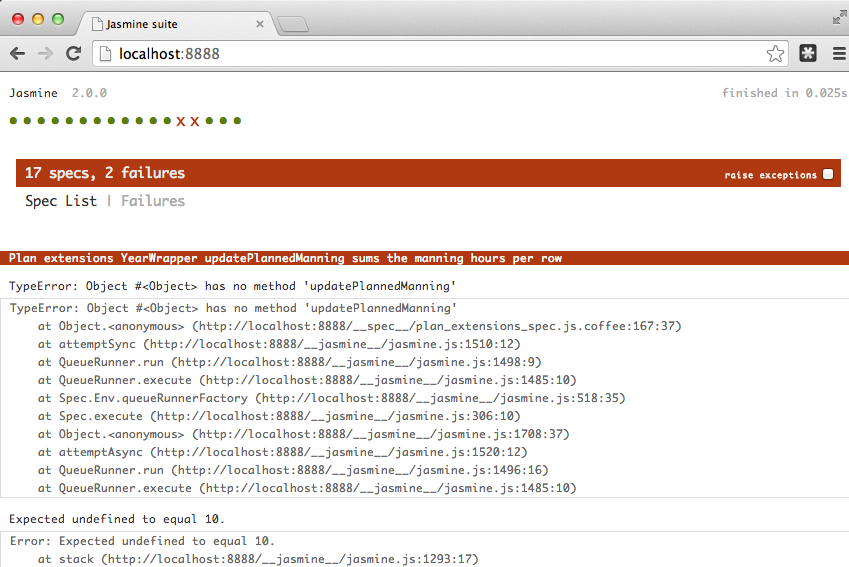
\includegraphics[width=0.8\textwidth]{methodology/jasmine_runner}
\caption{The test runner bundled with Jasmine.}
\label{fig:jasmine_runner}
\end{figure}

The Jasmine test runner did however have multiple issues. First of all,
it runs completely in the browser. Switching to the browser and reload
the page in order to run the tests are not excessively problematic, but
might be a little bit tiresome in the long run when using a test-driven
development methodology. A larger problem was the fact that the asset
handling, i.e. the compilation of CoffeeScript into Javascript, is
handled by Rails upon each reload. The used version of Rails re-compiles
all assets upon page load if any file has been changed. This process
takes a while, which means that each test run could take up to 10-15
seconds even though the actual tests only takes a fraction of a second
to run. The asset compilation also got stuck for for apparently no
reason once in a while. Since the server port on which the test runner
runs cannot be specified, it is also impossible to restart the test
runner without manually killing its system process.\\

Due to these issues, we switched to the Karma\footnote{\url{http
://karma-runner.github.io/}} test runner. Karma originates from a
master's thesis by \citet{article:karma}, and this covers several
problems with the Jasmine test runner as well as with some other
Javascript test runners. Karma was designed to solve several of these
issues and to be used with test-driven software methodologies. Tests are
run in a browser as soon as a file is changed, and the results are
reported back to the terminal and displayed as shown in
\fref{fig:karma_runner}. Re-compilation of source files and tests is
very fast and we did not experience any stability issues.\\

It took some effort with getting Karma to work with Rails, since it is
written in Node.js and does not have any knowledge about which
CoffeeScript files that exists in the Rails application. The task of
finding the location of all such files became more complex since
external Javascript libraries such as jQuery was loaded as Ruby gems,
and therefore not even located inside the project folder. We ended up
using a slightly modified version of a Rake script from a blog entry by
\citet{web:saunier_angular} for bootstrapping Karma in a Rails
environment. This script basically collects a list of filenames for all
Javascript assets by using Rails internal modules for asset handling,
and injects it into Karma's configuration file.\\

\begin{figure}
\centering
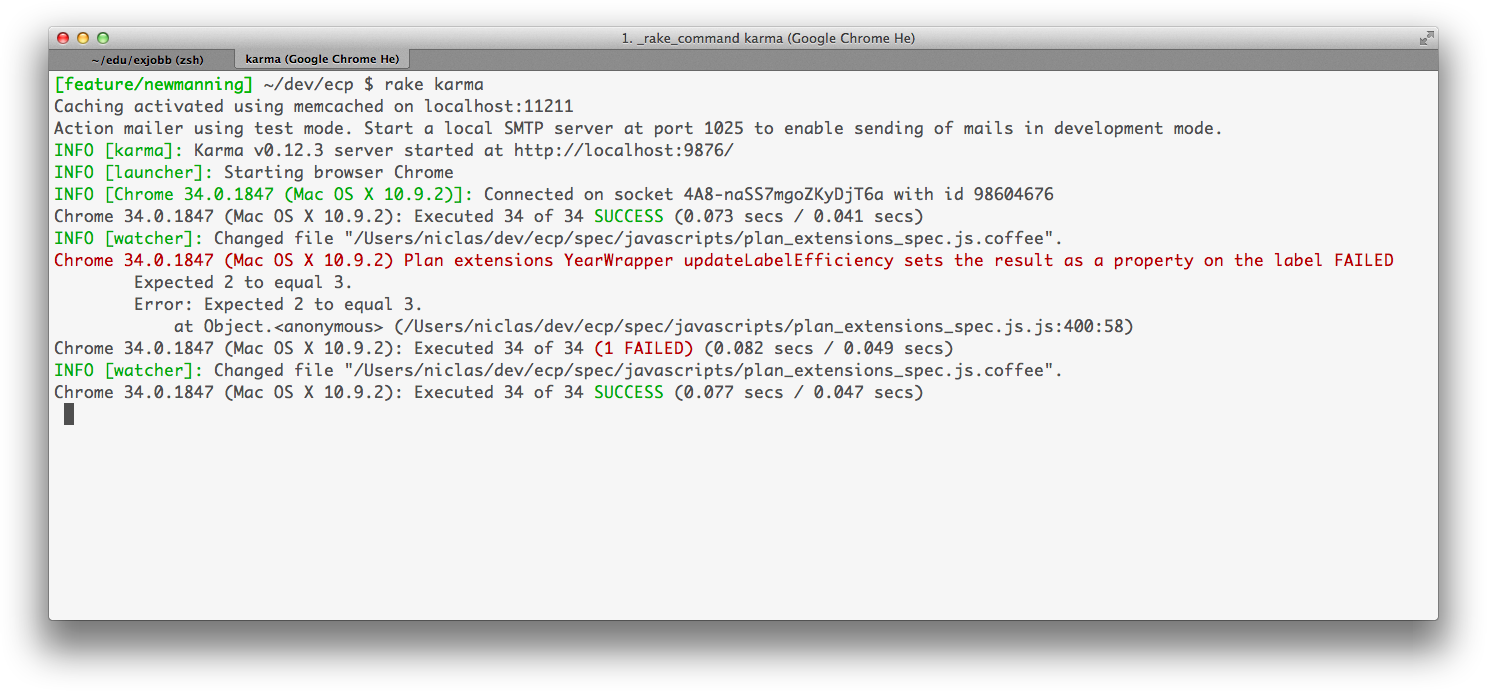
\includegraphics[width=0.8\textwidth]{methodology/karma_runner}
\caption{The Karma test runner.}
\label{fig:karma_runner}
\end{figure}


\subsection{Test coverage}
\label{sec:coverage_frameworks}

\subsubsection{Ruby test coverage}
There are multiple different ways of analyzing test coverage, and the
properties and conditions for each different kind of test coverage are
discoursed in \fref{sec:coverage}. However, we were unable to find any
test coverage tools for Ruby which analyzed anything else than statement
coverage, which is the weakest test coverage metric. Quite much effort
was spent on finding such tool, but without any success. Several
websites and Stack Overflow-answers indicates that no such tool exists
for Ruby at the time of this writing \cite{web:coverage_ruby19,
so:c1c2_coverage, so:c1_coverage, web:toolbox_code_metrics}. On one
hand, some of these sources are rather old and might be outdated, which
would indicate that such tool could have been created recently. On the
other hand would at least some of these sources probably been updated if
such tool became available.\\

We ended up using the
SimpleCov\footnote{\url{https://github.com/colszowka/simplecov}} tool
for Ruby test coverage metrics. At the time of this writing, it is the
most used Ruby tool for test coverage. It is also actively developed,
works with recent Ruby versions and RSpec versions, and produces pretty
and easy- to-read coverage reports in HTML (see
\fref{fig:simplecov_report}).\cite{web:toolbox_code_metrics}\\

\begin{figure}
\centering
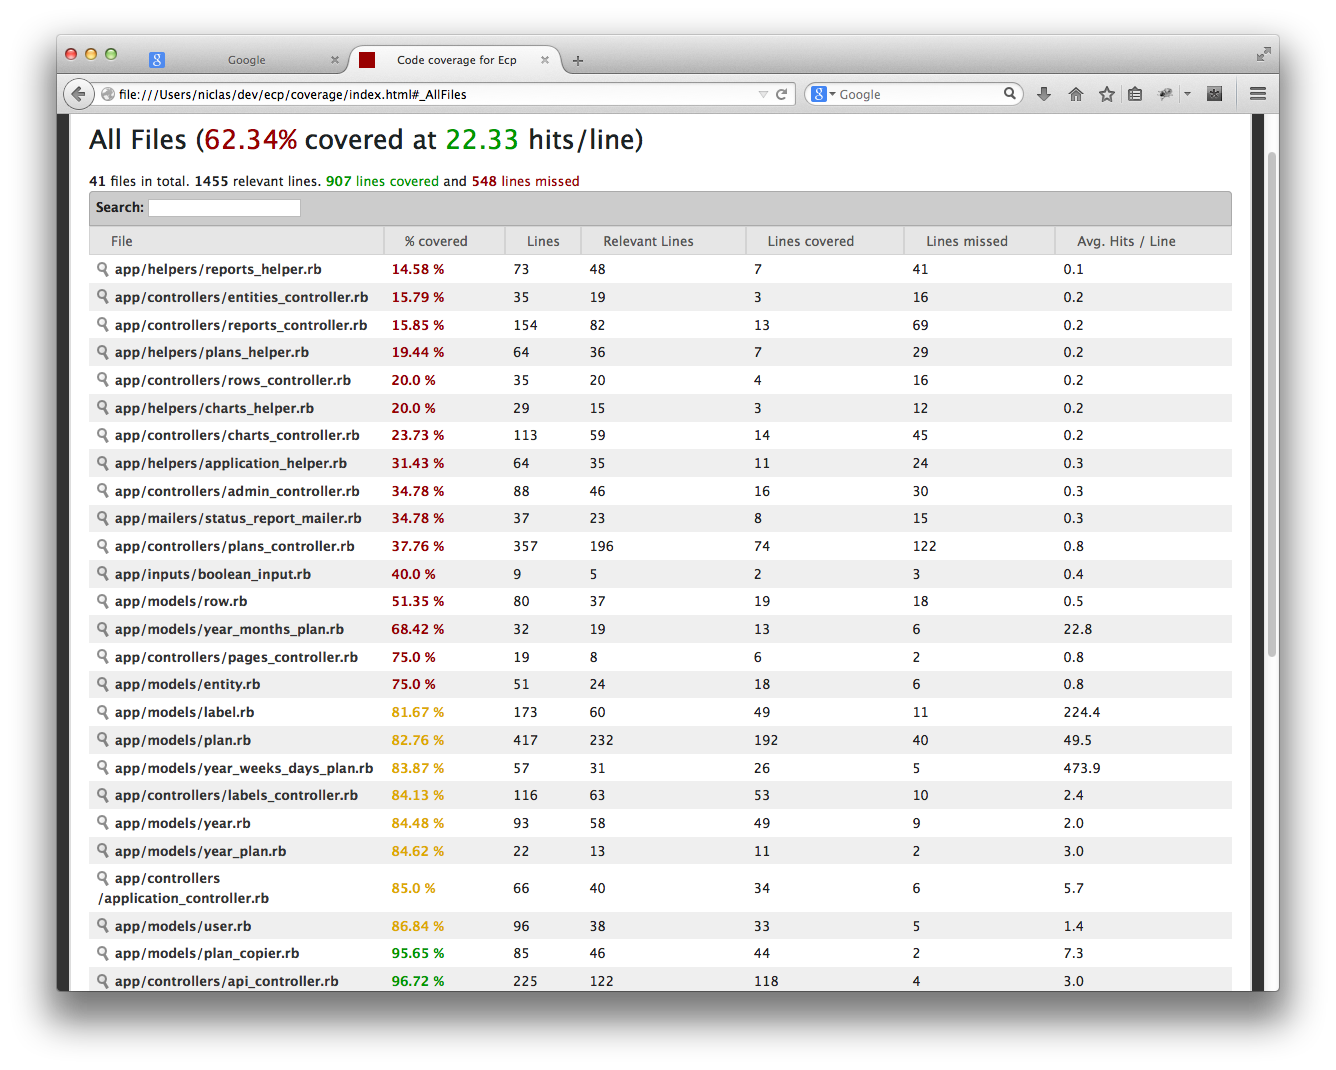
\includegraphics[width=0.8\textwidth]{results/simplecov}
\caption{A test coverage report generated by SimpleCov.}
\label{fig:simplecov_report}
\end{figure}


\subsubsection{CoffeeScript test coverage}
For the client-side CoffeeScript, we used a plug-in for the Karma test
runner called karma-coverage\footnote{\url{https://github.com/karma-
runner/karma-coverage}}. This tool basically integrates Karma with
Ibrik\footnote{\url{https://github.com/Constellation/ibrik}}, which is a
tool developed by Yahoo! for measuring test coverage of CoffeeScript
code. We did initially have some problems with getting this tool to work
correctly, since Ibrik internally uses another CoffeeScript compiler;
CoffeeScriptRedux, than the compiler used when tests itself are run.
CoffeeScriptRedux is more strict and yielded syntax errors in some of
our files, which could be compiled correctly in the production code. The
latest available release of Ibrik (version 1.1.1) also had major issues
with certain constructs in CoffeeScript, which made the files impossible
to analyze. This issues was however fixed in the development version.
Ibrik was first released in December 2013, which may explain its
immaturity. Ibrik internally uses istanbul-js for the coverage
analysis and report generation.\\

The chosen solution worked very well after sorting out the issues.
Statement coverage as well as branch coverage is supported, and it
yields useful reports. As with SimpleCov, the coverage reports are
produced as an interactive HTML report (see \fref{fig:karma_report}).\\

\begin{figure}
\centering
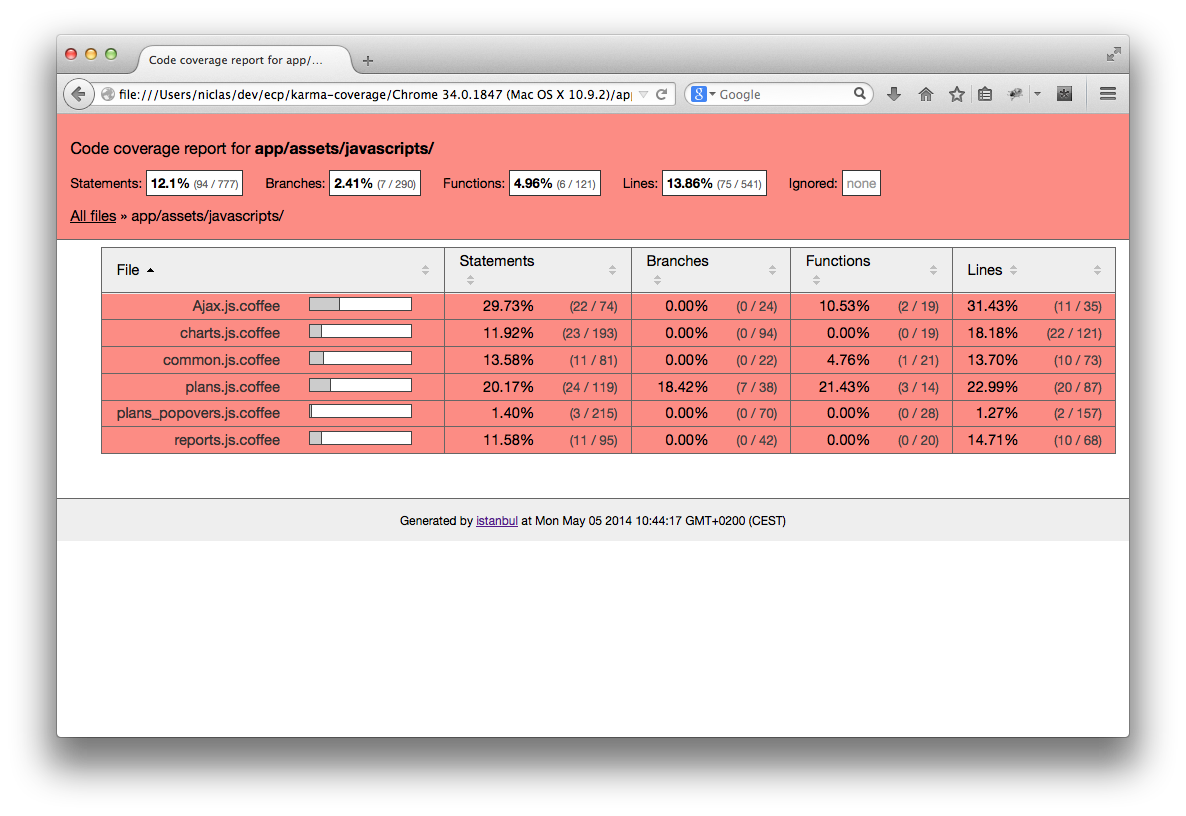
\includegraphics[width=0.8\textwidth]{methodology/karma_coverage}
\caption{A test coverage report generated by istanbul-js using karma-coverage.}
\label{fig:karma_report}
\end{figure}


\subsubsection{Test coverage issues}

One issue with using test coverage in this particular project is the
fact that very few files were added. Most of the changes was made in
existing classes and files, either as new functions or as changes to
existing functions. Since the overall test coverage is measured per
file, it is impossible to get an exact measure of how well-tested the
new and re-factored code is, since old and completely untested code
lower the test coverage.\\

We have tried to mitigate this by looking at the coverage reports by
hand, and try to determine a subjective measure of how good the test
coverage is for new and re-factored code. \Fref{fig:coverage_example}
shows an excerpt of a coverage report. In this case, our subjective
measure would say that the function |exports.getProduction()| is
completely untested. The function |exports.getLabelId()| is well tested
and has full statement- as well as branch coverage. The function
|exports.formatValues()| has full statement coverage, but non-optimal
branch coverage since the cases where |x| or |y| is not set are not
covered.\\

\begin{figure}
\centering
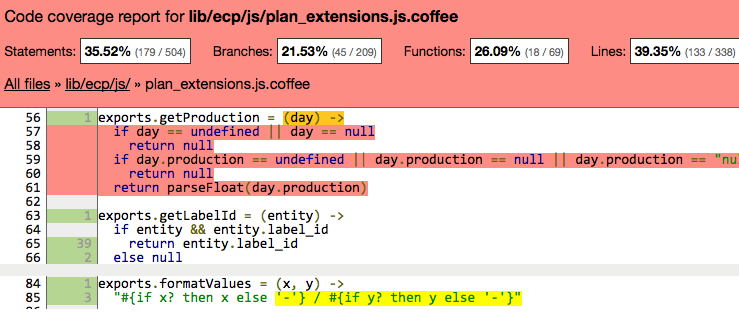
\includegraphics[width=0.8\textwidth]{results/js_coverage}
\caption{An excerpt from a coverage report generated using karma-coverage
         which demonstrates three different types of tested functions.}
\label{fig:coverage_example}
\end{figure}


\subsection{Mutation analysis}
\label{sec:choices_mutation}

There exists a few different tools for mutation analysis of Javascript
code. The ones we have found originates from academic research papers.
\citet{paper:mutandis} proposes a solution which has been implemented as
a tool called Mutandis
\footnote{\url{https://github.com/saltlab/mutandis/}}.
\citet{paper:ajaxmutator} presents another approach which has been
released as AjaxMutator \footnote{\url{https://github.com/knishiura-
lab/AjaxMutator}}. \citet{paper:webmujava} proposes a system-level
mutation testing approach called webMuJava.\\

Mutandis is based on website crawling tests. Although
\citeauthor{paper:mutandis} mentions that pure Javascript frameworks
have been tested using this tool, its implementation showed to be too
specific to be considered in our context. webMuJava does not seem to be
publicly available, and also seems to be too tightly integrated with a
specific back-end technique to be useful for Javascript-testing only.

AjaxMutator is in our opinion the most mature of all the considered
frameworks. It provides some basic documentation and installation
instructions, and the amount of implementation needed in order to begin
using it in a new project is reasonable. However, AjaxMutator currently
only supports Javascript tests written in Java using
JUnit\footnote{\url{http://junit.org/}}. Using it for mutation testing
tests written in CoffeeScript using Jasmine would probably be possible,
but the effort of doing this is outside the scope of this thesis.\\
